%!TEX root = main.tex
\section{Algebraic lattices and cryptographic applications}

%La troisième partie du cours sera effectuée par Alice Pellet-Mary. Après des
%éléments de théorie algébrique des nombres, elle définira les variantes
%algébriques de LWE et SIS, ainsi que le problème NTRU,
%et présentera leurs liens avec les réseaux algébriques. Elle construira alors
%des primitives cryptographiques élémentaires à partir de ces problèmes.
%Enfin, elle abordera des aspects de cryptanalyse et présentera des attaques
%exploitant la structure algébrique sous-jacente à ces problèmes.

In this section, we will discuss about structured lattices, and the corresponding structured variants of the LWE and SIS problem. We will also see a new algorithmic problem, called the NTRU problem.\footnote{This problem was originally defined as a structured lattice problem, and later generalized to a less structured (and even unstructured) version of itself.}

One of the main reason for introducing structure in lattices and lattice problems is to improve the efficiency of the cryptographic schemes based on lattices. Let's be clear here, schemes based on unstructured lattice problems such as (plain) LWE and SIS are \emph{not} inefficient, they are already somewhat efficient. But adding structure to the lattice can make them even more efficient, which makes everyone happier.
In order to see why the structure can make scheme more efficient, imagine that you have a lattice which has one basis $\vec B$ which is a circulant matrix, i.e., it is of the form
\begin{align*}
\vec B = \begin{pmatrix}
b_{1} & b_{2} & \dots & b_n \\
b_n & b_1 & \dots & b_{n-1} \\
\vdots & \ddots & \ddots & \vdots \\
b_{2} & b_3 & \dots & b_1
\end{pmatrix}.
\end{align*}
Then, storing this basis of you lattice only requires storing $n$ coefficients, instead of $n^2$ for an unstructured matrix. Also, multiplying this matrix with a vector can be done in quasi-linear time $O(n \cdot \poly( \log n) )$, instead of quadratic time $O(n^2)$.
Let's remark here that a structured lattice only need to have a few structured bases. Not all bases need to have this special structure (and in general, not all bases will have this visible structure indeed). But as long as we can compute a nicely structured basis, then we can enjoy the benefits of the structure on the storage space, and the running time of basic operations (like matrix-vector multiplication).

On the negative side, adding structure to the lattices may render the algorithmic problems based on these lattices easier to solve. From a cryptographic perspective, this would mean making the cryptographic constructions based on these problems weaker against attackers. It is then important to choose wisely the structure one adds to the lattices, and to study the impact of this structure on potential attacks.
There have been examples of poorly chosen structure, leading to attacks on the structured schemes \cite{BLA}.
%aller voir la thèse de Carl : https://www.esat.kuleuven.be/cosic/publications/thesis-399.pdf
% (une attaque de Gentry sur NTRU avec les sous corps de X^n-1, et ses propres articles sur le sujet)
On the other hand, we also have examples of good choice of structure,\footnote{Understand here that they are good \emph{so far}. They might become ``poorly chosen'' in a few months/years if someone manages to exploit the structure to find better attacks.} for which the best known attack is the same as the best known attack against unstructured lattices (i.e., for the moment, the only way we know to solve some algorithmic problems in these lattice is to forget about the structure, and use standard attacks against unstructured lattice problems).

The structure we will consider in this section is a special case of what is called \emph{modules over the ring of integers of a number field}. In order to make this name shorter, we will simply call these \emph{module lattices} in the rest of these lecture notes, as is commonly done in the cryptographic community. We will see in details what those objects are in Section~\ref{sec:number-theory} below. Module lattices are, by far, the most widely used structured lattices in lattice-based cryptography at the moment. If chosen appropriately, they may fall in the category of ``good structured lattices'' defined above, in the sens that, at the moment, we don't know how to solve standard algorithmic problems in these lattices (such at SVP) more efficiently than in non structured lattices.
Before moving to the formal definition of module lattices, let us mention the existence of other kinds of structured lattices (which won't be covered here), such as ideals over a maximal order of a cyclic algebra~\cite{CLWE}.


\subsection{Background on Number Theory}
\label{sec:number-theory}
In this section, we review some definitions and results of number theory that will be useful for the rest of the course. The last subsections are a little bit more advanced, and will be used only for the cryptanalysis part (Section~\ref{sec:cryptanalysis}). In this section, we will state most of the results without their proofs. Most of the proofs for the results about number theory can be found in Marcus' book~\cite{Marcus}. For the algorithmic results, or the results about modules, most of them are in Cohen's books~\cite{Cohen1, Cohen2}.
\subsubsection{Number fields}

A number field $K$ is a field, containing $\QQ$, and which has \emph{finite dimension} when seen as a vector space over $\QQ$.\footnote{Any field containing $\QQ$ can be seen as a vector space over $\QQ$, but not all of them have finite dimension as a $\QQ$-vector space. For instance, $\RR$ and $\CC$ are $\QQ$-vector spaces of infinite dimension.} The dimension of $K$ over $\QQ$ is called the \emph{degree} of the number field $K$, and denoted by $[K:\QQ]$. In these lecture notes, by convention, we will use the letter $d$ to denote the degree of a number field (when there is no conflict of notation).

There are multiple ways to represent number fields. The most frequent ones are seeing them as subsets of $\CC$, or as polynomial rings. In these lecture notes, we will adopt the polynomial ring representation, which will be more convenient.

\begin{lemma}
\label{le:nb-field-eq-def}
Let $P \in \QQ[X]$ be an irreducible polynomial of degree $d$. Then the polynomial ring $\QQ[X]/P(X)$ is a number field of degree $d$.
Conversely, if $K$ is a number field of degree $d$, then there exists an irreducible polynomial $P$ of degree $d$ such that $K$ is isomorphic (as a field) to $\QQ[X]/P(X)$.
\end{lemma}

In the rest of these lecture notes, let us fix an irreducible monic polynomial $P$ of degree $d$, and define $K = \QQ[X]/P(X)$. Note that for any polynomial $f(X) \in \QQ[X]$, there is a unique polynomial $g(X) \in \QQ[X]$ with degree $< d$ and such that $f(X) = g(X) \bmod P$. We will represent elements of $K$ by the unique representative of their class which has degree $< d$. In other words, we see $K$ as the set $\{\sum_{i = 0}^{d-1} x_i X^i\,|\, x_i \in \QQ\}$ (where operations are performed modulo $P$). With this representation, we see that $\QQ$ is indeed contained in $K$, as the set of all polynomials of degree $0$.

\begin{example}\ 
\begin{enumerate}
\item Taking $P = 1$ leads to $K = \QQ$, the simplest of all number field. This is not a very interesting one, but keeping it in mind can be useful sometimes, to gain some intuition about what is happening.
\item A very common choice of polynomial $P$ in cryptography is $P = X^d+1$, where $d$ is a power-of-two. This polynomial is a cyclotomic polynomial (its roots are the primitive $(2d)$-th roots of unity), and the field $K$ associated to it is called a cyclotomic field. Cyclotomic fields have been extensively studied and they enjoy nice properties, that can be useful in cryptography, both for constructing cryptographic primitives, and for cryptanalysis. Most of the schemes using structured lattices today rely on power-of-two cyclotomic fields.
\item An other famous choice of polynomial is $P = X^p-X-1$, with $p$ a prime number. These polynomials are used in the NTRU Prime construction~\cite{NTRUPrime}, and we will call the associated field $K$ an NTRU Prime field. An interesting property of these fields is that they have no subfields, i.e., there exist no field $L$ such that $\QQ \varsubsetneq L \varsubsetneq K$.
\end{enumerate}
\end{example}

\paragraph{Ring of integers.} A number field $K$ contains a special sub-ring, called the \emph{ring of integers} of the number field (also called sometimes the maximal order of the number field). It is defined as follows.

\begin{definition}
\label{def:ring-of-integers}
Let $K$ be a number field. The ring of integers $\O_K$ of $K$ is the subset of $K$ formed by all the elements that are integral over $\ZZ$, i.e., all elements $x$ of $K$ such that there exists a monic irreducible polynomial $P_x \in \ZZ[X]$ satisfying $P_x(x) = 0$.
\end{definition}

It can be proven that this set $\O_K$ is indeed a ring (but not a field). Moreover, $\O_K$ is a $\ZZ$-module of rank $d$, i.e., there exists $d$ elements $\alpha_1, \dots, \alpha_d \in \O_K$ such that any element $x \in \O_K$ can be uniquely written as $x = \sum_i x_i \alpha_i$, with $x_i \in \ZZ$. Such elements $(\alpha_1, \dots, \alpha_d)$ also form a $\QQ$-basis of the $\QQ$-vector space $K$. They are called an \emph{integral basis} of $K$.

\begin{example}\ 
\begin{enumerate}
\item If $K = \QQ$, then $\O_K = \ZZ$, and $(1)$ is an integral basis of $K$.
\item If $K = \QQ[X]/(X^d+1)$ with $d$ a power-of-two, then $\O_K = \ZZ[X]/(X^d+1)$. Moreover, $(1,X, \dots, X^{d-1})$ is an integral basis of $K$.
\item In full generality, if $K = \QQ[X]/P(X)$ with $P$ irreducible, then $\ZZ[X]/P(X) \subseteq \O_K$, but we might not have equality.
\end{enumerate}
\end{example}

One of the consequence of the existence of integral bases is that elements of $K$ can be seen as fractions, with numerators in $\O_K$ and denominators in $\ZZ$ (by default, the denominators would have been in $\O_K$ too), as stated in the following lemma.
\begin{lemma}
Any $x \in K$ can be written as $x = \frac{z}{n}$ with $z \in \O_K$ and $n \in \ZZ_{>0}$.
\end{lemma}
\begin{proof}
Take an integral basis $(\alpha_1, \dots, \alpha_d)$ of $K$ and let $x_i \in \QQ$ be such that $x = \sum_i x_i \alpha_i$. Then taking $n$ to be the least common multiple of all the denominators of the $x_i$'s gives the desired result.
\end{proof}

\paragraph{Complex embeddings.} There exists always $d$ fields homomorphisms from $K$ to $\CC$,\footnote{We impose here that the field homomorphism sends $1$ to $1$, which avoids the trivial function sending every element of $K$ to $0$.} called the \emph{complex embeddings} of $K$. Note that field homomorphisms are always injective, and that they fix $\QQ$ point-wise. Let us write $\sigma_1, \dots, \sigma_d$ these complex embeddings. Some of them may have their image lying fully in $\RR \subset \CC$. We call those real embeddings, and we will write $d_\RR$ their number. If $\sigma$ is a complex embedding whose image is not fully contained in $\RR$, then $\overline{\sigma}$ (defined by $\overline{\sigma}(x) = \overline{\sigma(x)}$) is also a complex embedding. We say that $\sigma$ and $\overline{\sigma}$ are conjugate. Let $d_{\CC}$ be the number of such pairs of conjugate complex embeddings. Then we have $d = d_\RR + 2 d_\CC$. In the rest of this course, we order the complex embeddings such that $\sigma_1, \dots, \sigma_{d_\RR}$ are real embeddings, and $(\sigma_i, \sigma_{i+d_\CC})$ are pairs of conjugate embeddings for $d_\RR < i \leq d_\RR+d_\CC$.

\begin{lemma}
Let $K = \QQ[X]/P(X)$ with $P$ irreducible, and let $\alpha_1, \dots, \alpha_d$ be the $d$ roots of $P$ in~$\CC$. Then, the complex embeddings of $K$ are exactly the functions
\begin{align*}
\sigma_i: \ \ \ K & \rightarrow \CC \\
                f(X) & \mapsto f(\alpha_i)
\end{align*}
for $i \in \{1, \dots, d\}$.\footnote{Here, $f$ is a polynomial in $\QQ[X]$ of degree $< d$. We use the fact that $P(\alpha_i) = 0$, which implies that reduction modulo $P$ does not change the output of the function, and so the function is well defined over $\QQ[X]/P(X)$.}
\end{lemma}

\begin{proof}
First of all, one can check that the functions $\sigma_i$ defined in the lemma are indeed field homomorphisms, with image in $\CC$, as desired. Moreover, since $P$ is irreducible, then all the roots $\alpha_i$ are distinct, and so the functions $\sigma_i$ are distinct too (since they have distinct evaluations at~$X$).

If we admit that there are only $d$ complex embeddings for $K$, then we are done. However, since the proof is instructive, we will also prove that any complex embedding of $K$ is one of the~$\sigma_i$. This will also prove that there are exactly $d$ complex embeddings (which we have admitted above).

Let $\sigma$ be a complex embedding. Since it is a field homomorphism and since it fixes $\QQ$, then the knowledge of $\sigma(X)$ uniquely determines $\sigma$. Indeed, if $\beta = \sigma(X) \in \CC$, then for any $f(X) = \sum_i f_i X^i \in K$ (with $f_i \in \QQ$), we have $\sigma(\sum_i f_i X^i) = \sum_i f_i \beta^i = f(\beta)$.
Moreover, since $P(X) = 0$, then we should have $P(\beta) = P(\sigma(X)) = \sigma(P(X)) = \sigma(0) = 0$. So $\beta$ is a complex root of $P$, i.e., it is one of the $\alpha_i$'s. This proves that $\sigma$ is equal to one of the $\sigma_i$'s.
\end{proof}

\begin{example}
If $K = \QQ[X]/(X^d+1)$ with $d$ a power-of-two, then $d_\RR = 0$, $d_\CC = d/2$ and the $d$ complex embeddings of $K$ are obtained by sending $X$ to all the primitive $(2d)$-th roots of unity in $\CC$ (there are $\varphi(2d) = d$ such primitive roots, which are exactly the roots of $X^d+1$).
\end{example}

\paragraph{Trace and norm.} The trace $\Tr$ and algebraic norm $\N$ are functions from $K$ to $\CC$ defined as follows. For any $x \in K$
\begin{align*}
\Tr(x) &= \sum_{i = 1}^d \sigma_i(x) \\
\N(x) &= \prod_{i = 1}^d \sigma_i(x)
\end{align*}
\begin{lemma}
For any $x \in K$, the trace and the norm of $x$ are in $\QQ$ (and not only in $\CC$). Moreover, if $x \in \O_K$, then $\Tr(x)$ and $\N(x)$ are in $\ZZ$.
\end{lemma}

\begin{example}
If $K = \QQ[X]/(X^2+1)$ and $x = a+bX$, then
\begin{align*}
\Tr(x) &= (a+ib) + (a-ib) = 2a \\
\N(x) &= (a+ib) \cdot (a-ib) = a^2+b^2
\end{align*}
\end{example}

\begin{lemma}
The trace is additive and the algebraic norm is multiplicative. I.e., for any $x, y \in K$, it holds that
\begin{align*}
\Tr(x+y) &= \Tr(x) + \Tr(y) \\
\N(xy) &= \N(x) \cdot \N(y)
\end{align*}
\end{lemma}

\subsubsection{Ideals} For any commutative ring $R$, an \emph{ideal} $I$ of $R$ is a subset of which is an additive group, and is stable by multiplication by an element of $R$, i.e., for all $x \in I$ and $\alpha \in R$, it holds that $\alpha x \in I$. In our context with number fields $K$ and ring of integers $\O_K$, we will consider ideals of $\O_K$, as well as a generalization of those.

\begin{definition}
Let $K$ be a number field and $\O_K$ its ring of integers.
\begin{itemize}
\item An \emph{integral ideal} of $K$ is an ideal of $\O_K$, for the definition given above. By convention, we will use Gothic letters $\mathfrak{a}, \mathfrak{b}, \cdots$ to denote integral ideals.
\item A \emph{fractional ideal} of $K$ is a subset $I \subset K$ of the form $x \cdot \mathfrak{a} := \{x \cdot a\,|\, a \in \mathfrak{a}\}$ for some $x \in K^*$ and $\mathfrak{a}$ an integral ideal of $K$. By convention, we will use capital letters $I, J, \cdots$ to denote fractional ideals.
\end{itemize}
\end{definition}

Note that $K$ is a ring, and so one can define the ideals of $K$ when seen as a ring. However, since $K$ is also a field, it only has two ideals: $K$ and $\{0\}$. Those are not very interesting, and we will never consider ideals of $K$ in these lecture notes. Instead, we will sometimes use the terminology ``ideal of $K$'' to refer to fractional ideals of $K$ (and we will always specify ``\emph{integral} ideal if $K$'' when they are integral).

\begin{example}
For $K = \QQ$ and $\O_K = \ZZ$, the set $\mathfrak{a} = \{3x\,|\, x \in \ZZ\}$ is an integral ideal of $K$. And the set $I = \{5x/7 \,|\, x \in \ZZ\}$ is a fractional ideal of $K$.
\end{example}

\begin{definition}
A fractional ideal $I$ of $K$ is said to be \emph{principal} if it is of the form $\alpha \O_K := \{ \alpha \cdot x\,|\, x \in \O_K\}$ for some $\alpha \in K$. In this case, $\alpha$ is called a \emph{generator} of $I$ (it is usually not unique).
\end{definition}

\begin{example}
The two ideals from the previous example are principal, with generators $3$ and $5/7$ respectively. This is not a coincidence, all ideals in $\ZZ$ are principal, we say that $\ZZ$ is a principal ideal domain (PID).
In general, the ring $\O_K$ may not be principal, meaning that there exists ideals that are not generated by a single element.
\end{example}

\begin{lemma}
\label{lemma:two-elm-rep}
Any fractional ideal $I$ can be generated by at most $2$ elements of $K$, i.e., there exists $\alpha, \beta \in K$ such that $I = \{ \alpha \cdot x + \beta \cdot y \,|\, x, y \in \O_K\}$.
\end{lemma}

\paragraph{Arithmetic over ideals.} In a number field $K$, we will want to do arithmetic over the fractional ideals. We will see below that, while the ring $\O_K$ might not have the same nice arithmetic properties as the ring $\ZZ$ (for instance, we usually do not have euclidean division in $\O_K$, and sometimes not even unique factorization), everything works better if we consider ideals of $\O_K$, rather than elements of $\O_K$.

\begin{definition}
Let $I$ and $J$ be two fractional ideals. We define the addition and multiplication of $I$ and $J$ as
\begin{align*}
I + J &= \{x + y \,|\, x \in I, y \in J\} \\
I \cdot J &= \{ \sum_{i = 1}^r x_i \cdot y_i \,|\, r > 0, x_i \in I, y_i \in J\}.
\end{align*}
\end{definition}

\begin{example}
When $K = \QQ$ and $\O_K = \ZZ$, we have $6\ZZ + 8 \ZZ = 2\ZZ$, and $2 \ZZ \cdot 3 \ZZ = 6 \ZZ$.

When the ideals are integral, the addition of two ideals corresponds to their gcd, i.e., if $x, y \in \ZZ$, then $x \ZZ + y \ZZ = \gcd(x,y) \ZZ$. More generally, in an arbitrary number field $K$, the sum of two integral ideals $\mathfrak{a}$ and $\mathfrak{b}$ is the smallest (for inclusion) integral ideal containing both $\mathfrak{a}$ and $\mathfrak{b}$.

In any number field $K$, if $I = \alpha \O_K$ and $J = \beta \O_K$ are principal, then we always have $I\cdot J = (\alpha \cdot \beta)\O_K$.
\end{example}

\begin{lemma}
The sum and product of two fractional ideals is still a fractional ideal. Moreover, the set of non-zero fractional ideal forms a multiplicative group with neutral element $\O_K$, i.e., for any non-zero fractional ideal $I$, there exists a non-zero fractional ideal $J$ such that $I \cdot J = \O_K$. This ideal $J$ is called the inverse of $I$, and we write it $I^{-1}$.
\end{lemma}

There exists also a notion of prime ideals in $K$.

\begin{definition}
A \emph{prime ideal} $\mathfrak{p}$ of $K$ is an \emph{integral} ideal such that for any two elements $\alpha, \beta \in \O_K$, if $\alpha \cdot \beta \in \mathfrak{p}$, then it must be that either $\alpha \in \mathfrak{p}$ or $\beta \in \mathfrak{p}$.
We will also assume in these lecture notes that a prime ideal is non-zero.\footnote{The convention usually consists in accepting $\{0\}$ as a prime ideal, and writing everywhere ``non-zero prime ideal''. We exclude $\{0\}$ from the beginning to avoid unnecessary heavy notations.}
\end{definition}

\begin{example}
Over $\ZZ$, the prime ideals are exactly the ideals $p \cdot \ZZ$, where $p$ is a prime integer.

In $K = \QQ[X]/(X^2+1)$ and $\O_K = \ZZ[X]/(X^2+1)$, the principal ideal $\mathfrak{a} := (1+X) \cdot \O_K$ is prime. To see this, one can first check that an element $a + bX \in \O_K$ is divisible by $1+X$ if and only if $a = b \bmod 2$. Hence, $\mathfrak{a} = \{a + bX \,|\, a, b \in \ZZ, a = b \bmod 2\}$. Let $x = a+bX$ and $y = c+dX$ be in $\O_K$ and such that $x \cdot y \in \mathfrak{a}$. We have $x \cdot y = (ac-bd) + (ad+bc)X$, and so by the property above, we know that $ac-bd = ad+bc \bmod 2$. One can check that this equation implies that either $a = b \bmod 2$ or $c = d \bmod 2$ (for instance, by testing all the $2^4$ possible values of $a,b,c$ and $d$ modulo $2$). Hence, either $x$ of $y$ is in $\mathfrak{a}$, as desired.
\end{example}

\begin{lemma}
Any \emph{integral} ideal of $K$ can be factored in a unique way (up to permutation of the terms) as a product of prime ideals. In other words, for any integral ideal $\mathfrak{a}$, there exists a unique sequence of non-negative integers $(n_\mathfrak{p})_{\mathfrak{p}}$, ranging over all prime ideals and non-zero only for a finite number of prime ideals, such that $\mathfrak{a} = \prod_{\mathfrak{p}} \mathfrak{p}^{n_\mathfrak{p}}$.

\noindent For fractional ideals $I$, there is also a unique factorization, but exponents may be negative, i.e., $I = \prod_{\mathfrak{p}} \mathfrak{p}^{x_\mathfrak{p}}$ where $x_\mathfrak{p} \in \ZZ$ is zero for almost all primes.
\end{lemma}

\begin{example}
In $K = \QQ[X]/(X^2+1)$, we have $2 \O_K = \mathfrak{p}^2$, where $\mathfrak{p} = (1+X) \cdot \O_K$ is the prime ideal from the previous example. To see this, note that $(1+X)^2 = 2X \bmod X^2+1$, so $\mathfrak{p}^2 = (2X) \cdot \O_K$. But since $X$ is inertible in $\O_K$ (with inverse $-X$), the ideals $(2X) \cdot \O_K$ and $2 \O_K$ are equal.
\end{example}

\begin{lemma}
An integral ideal $\mathfrak{a}$ is prime if and only if the quotient space $\O_K/\mathfrak{a}$ has no divisors of zero. In our case, this is equivalent to $\O_K/\mathfrak{a}$ being a field (because it is a finite, commutative ring).
\end{lemma}

\paragraph{Algebraic norm.} The algebraic norm of an non-zero integral ideal $\mathfrak{a}$ is $\N(a) = |\O_K/\mathfrak{a}|$, i.e., it is the index of $\mathfrak{a}$ in $\O_K$. This is an positive integer. For a non-zero fractional ideal $I = x \cdot \mathfrak{a}$, with $x \in K$ and $\mathfrak{a}$ an integral ideal, the algebraic norm is defined as $\N(I) = |\N(x)| \cdot |\N(\mathfrak{a})|$. This is a positive rational number, and it does not depend on the choice of $x$ and $\mathfrak{a}$.

\begin{properties}
\label{prop:norm-ideal}
\begin{enumerate}
\item if $I = \alpha \O_K$ is principal, then $\N(I) = |\N(\alpha)|$;
\item the norm is multiplicative, i.e., for $I$ and $J$ fractional ideals, we have $\N(I \cdot J) = \N(I) \cdot \N(J)$;
\item if $\mathfrak{p}$ is a prime ideal, then $\N(\mathfrak{p}) = p^k$ for some $k \geq 1$ and $p$ a prime integer;
\item for an integral ideal $\mathfrak{a}$, we have $\N(\mathfrak{a}) \in \mathfrak{a}$ (when seeing $\N(\mathfrak{a})$ as an element of $K$ via the inclusion $\ZZ \subset K$).
\end{enumerate}
\item if $I \subseteq J$, then $I = \mathfrak{a} \cdot J$ with $\mathfrak{a}$ a fractional ideal. This implies in particular that $\N(J) |\N(I)$ (because $\N(\mathfrak{a})$ is an integer).
\end{properties}


\paragraph{Computational aspects.} {\color{red} TODO}$\ZZ$-basis of ideals. The fact that we can go from $2$-elements representation to basis in polynomial time and conversely. The fact that we can add and multiply efficiently, and factor ideals if we can factor integers.

\subsubsection{Modules}
\label{sec:modules}
Let $m \geq 1$ be an integer and let $M \subset K^m$. We say that $M$ is a finitely generated $\O_K$-module if and only if there exists vectors $\vec b_1, \cdots, \vec b_t \in K^m$ such that
\[ M = \{ \sum_{i = 1}^t x_i \vec b_i \,|\, x_1, \dots, x_t \in \O_K\}. \]
We say that such elements $(\vec b_1, \dots, \vec b_t)$ are a generating set of $M$ (they are not unique).
In the rest of these lecture notes, we will say that $M$ is a ($\O_K$-)module, instead of the longer (but more accurate) terminology ``finitely generated $\O_K$-module included in $K^m$ for some $m \geq 1$''.

\begin{lemma}
If $m = 1$, then a $M \subset K$ is a module if and only if it is a fractional ideal of $K$.
\end{lemma}
\noindent Ideals are the simplest cases of modules, when the dimension is $1$.

\begin{proof}
Let $I$ be a fractional ideal. From Lemma~\ref{lemma:two-elm-rep}, we know that $I = \{ x_1 \alpha + x_2 \beta \,|\, x_1, x_2 \in \O_K\}$ for some $\alpha, \beta \in K$. This proves that $I$ is a module in $K$ for our definition above.
On the other hand, let $M \subset K$ be a module. By definition, there exists $b_1, \dots, b_t \in K$ such that $M = b_1 \O_K + \dots + b_t \O_K$. In other words, $M$ is the sum of all the principal ideals $b_i \O_K$. We have seen that a sum of ideals is still an ideal, which concludes the proof.
\end{proof}

\begin{definition}
The rank of a module $M$ is the dimension of the $K$-vector space spanned by the elements of $M$ (which is a subspace of $K^m$).
\end{definition}

By setting $K = \QQ$ and $\O_K = \ZZ$, one can see that a $\ZZ$-module is simply a lattice. In a sense, modules are generalizations of lattices, to more general rings (here, the ring $\O_K$). There are still some differences between modules and lattices. The first one is that, in lattices, we often care about geometric questions. For this, we need to have a notion of ``size'' for the vectors of our lattice, which is obtained by taking their euclidean norm (or infinity norm, or any other norm). When replacing $\QQ$ by $K$, it is nor clear anymore what the size of an element of $K$ is, let alone a vector of $K^m$. We will discuss this in more details in Sections~\ref{sec:embeddings} and~\ref{sec:id-mod-lat}.

Another difference between modules and lattices is that lattices always have bases, but modules may not. So far, we have defined a module by a generating set, but it might not be possible to extract a set of linearly independent basis vectors from this generating set. There exists however a notion of pseudo-basis, which can be used somehow analogously to the notion of basis (up to some more technicalities).

\begin{lemma}
Let $M$ be a module of rank $r$ included in $K^m$. There exists $r$ vectors $\vec b_1, \dots, \vec b_r \in K^m$ that are $K$-linearly independent, and $r$ fractional ideals $I_1, \dots, I_r$ such that
\[ M = \sum_{i = 1}^r I_i \cdot \vec b_i := \{ \sum_i x_i \vec b_i \,|\, x_i \in I_i \text{ for all }i\}.\]
The list of pairs $\big((\vec b_i, I_i)\big)_{1 \leq i \leq r}$ is called a \emph{pseudo-basis} of the module $M$.
\end{lemma}

\begin{definition}
When $M$ admits a pseudo-basis $\big((\vec b_i, I_i)\big)_{1 \leq i \leq r}$ with all ideals $I_i$ equal to $\O_K$, we say that $M$ is free.
\end{definition}
When $I_i = \O_K$ for all $i$'s, then the $\vec b_i$'s form a basis of $M$, for the usual definition of a basis (any element of $M$ can be uniquely written as a linear combination over $\O_K$ of those vectors). Observe that, in our definition, the module $M$ is free if \emph{at least one} of its pseudo-basis is a basis, but we do not require that all pseudo-bases have $I_i = \O_K$ (this would not be possible anyway).

\subsubsection{Embeddings}
\label{sec:embeddings}
We have seen above that it would be convenient to be able to define a notion of ``size'' of an element of $K$ (which we would then extend to a notion of ``size'' for the vectors of $K^m$). A usual way to obtain this is to embed $K$ into $\CC^d$, and then use, e.g., the hermitian norm over $\CC$, or the infinity norm. There are two frequently used embeddings of $K$ into $\CC^d$, leading to two different notions of size for a elements of $K$.

\begin{definition}
Let $K = \QQ[X]/P(X)$ be a number field. The coefficient embedding of $K$ is defined as
\begin{align*}
\coeff: \hspace{15mm} K & \rightarrow \QQ^d \\
\sum_{i=0}^{d-1} a_i X^i &\mapsto	(a_0, \dots, a_{d-1}),
\end{align*}
and the canonical embedding (or Minkowski's embedding) is defined as
\begin{align*}
\mink: \hspace{4mm} K & \rightarrow \CC^d \\
x &\mapsto	(\sigma_1(x), \dots, \sigma_d(x)),
\end{align*}
where $\sigma_1, \dots, \sigma_d$ are the complex embeddings of $K$, defined above.
\end{definition}

Note that the canonical embedding depends on our choice of polynomial $P$. If we use a different polynomial $P'$ defining an isomorphic number field $K'$, then the coefficient embedding can change, whereas the canonical embedding will stay the same (up to permutation of the coordinates, which are not uniquely ordered).

\begin{example}
In $K = \QQ[X]/(X^2+1)$, we have $\coeff(1+X) = (1,1) \in \QQ^2$ and $\mink(1+X) = (1+i, 1-i) \in \CC^2$.
\end{example}

One of the advantage of the coefficient embedding is that it lives in $\QQ^d$ instead of $\CC^d$, which makes it easier to manipulate on a computer. On the other hand, the canonical embedding is more intrinsic to the field, and enjoy nicer mathematical properties, which can be useful for analysis.

Let's also remark that the image of $\mink(K)$ lives in a $\RR$-vector subspace of $\CC^d$, with dimension $d$ over $\RR$ (when $\CC^d$ has dimension $2d$ over $\RR$). This is the space
\[\{x \in \CC^d \,|\, x_1, \dots, x_{d_\RR} \in \RR, \text{ and } x_{d_\RR+1} = \overline{x_{d_\RR+d_\CC+1}}, \dots, x_{d_\RR+d_\CC} = \overline{x_d} \}.\]

Now that we have functions to embed $K$ into $\CC^d$, we can define the ``size'' of an element of $K$ as the euclidean norm of its coefficient embedding, or of its canonical embedding. This usually gives different notion of sizes, but in the specific case of power-of-two cyclotomic field, one can prove that both notions are strongly related.

\begin{proposition}
Let $K = \QQ[X]/X^d+1$ with $d$ a power-of-two. Then for all $x \in K$, we have $\|\mink(x)\| = \sqrt{d} \cdot \|\coeff(x)\|$.
\end{proposition}
In this specific case, the canonical embedding is a scaled isometry of the coefficient embedding. For other cyclotomic fields, one can also relate the coefficient and canonical embeddings, but those are usually not scaled isometries of one another (see, e.g.,~\cite{Blanco}).

Finally, let us introduce some convenient notation: for $\vec b = (b_1, \dots, b_m)^T \in K^m$, we will write $\mink(\vec b) = (\mink(b_1), \dots, \mink(b_m))^T \in \CC^{dm}$. Similarly, we write $\coeff(\vec b) \in \QQ^{dm}$ for the application of $\coeff$ coordinate-wise.

\paragraph{Some useful properties.} As said above, the canonical embedding enjoys nice mathematical properties. One of them is that it can be related to the algebraic norm.

\begin{lemma}
\label{lemma:AM-GM-inequality}
Let $x \in K$, then $\|\mink(x)\| \geq \sqrt{d} \cdot |\N(x)|^{1/d}$. In particular, for any $x \in \O_K$ non-zero, we have $\|\mink(x)\| \geq \sqrt{d}$.
\end{lemma}

\begin{proof}
Applying the inequality of arithmetic and geometric means to the vector $(|\sigma_1(x)|^2, \dots, |\sigma_d(x)|^2)$ leads
\[ 1/d \cdot \|\mink(x)\|^2 = 1/d \cdot \sum_i |\sigma_i(x)|^2 \geq \Big(\prod_i |\sigma_i(x)|^2\Big)^{1/d} = |\N(x)|^{2/d},\]
which gives the desired inequality. The second part of the statement is obtained by noticing that the algebraic norm of an non-zero element of $\O_K$ is an integer, thus it is $\geq 1$ in absolute value.
\end{proof}

The norm induced over $K$ by the canonical embedding satisfies the triangular inequality (which is a requirement for a norm), but it is also sub-multiplicative.

\begin{lemma}
For any $x,y \in K$, we have
\[\|\mink(x \cdot y)\| \leq \|\mink(x)\|_\infty \cdot \|\mink(y)\| \leq \|\mink(x)\| \cdot \|\mink(y)\|.\]
\end{lemma}

\begin{proof}
This properties follows from the fact that, by definition of $\mink$, the vector $\mink(x \cdot y)$ is the product coordinate-wise of the vectors $\mink(x)$ and $\mink(y)$.
\end{proof}

\subsubsection{Ideal and module lattices}
\label{sec:id-mod-lat}
Ideal and module lattices are ideals and modules to which we add a lattice structure, by using one of the embeddings defined above.

\begin{proposition}
Let $M$ a module in $K^m$ of rank $r$. Then, the sets 
\[\coeff(M) := \{ \coeff(\vec b)\,|\, \vec b\in M\} \subset \QQ^{md}\]
and 
\[\mink(M) := \{ \mink(\vec b)\,|\, \vec b\in M\} \subset \CC^{md}\]
are lattices of rank $dr$.\footnote{Note that we usually define a lattice as a subset of $\RR^t$, but our set $\mink(M)$ lives in $\CC^{md}$. Extending the definition of lattices to subset of $\CC^t$ (using the hermitian norm of $\CC$) is usually pretty harmless, but if one prefers to keep all lattices in $\RR^t$, it suffices to map $\CC^{md}$ to $\RR^{2md}$ isometrically, and consider $\mink(M)$ as a (non full-rank) lattice in this space.}
They are called \textit{module lattices}. If $m = r = 1$, then $M = I$ is a fractional ideal, and we call $\coeff(I)$ and $\mink(I)$ ideal lattices.
\end{proposition}

Since $\O_K$ is an ideal, the proposition above also applies to it, and we have that $\mink(\O_K)$ is a lattice of rank $d$. Its volume square $\det(\mink(\O_K))^2$ is a quantity called the \textit{discriminant} of the number field $K$, and written $\Delta_K$.\footnote{With our definition, the discriminant of a number field is always $> 0$, since the volume $\det(L)$ of a lattice is. In math textbooks, the definition of the discriminant is usually slightly different, and our definition corresponds to the absolute value of the usual definition.}

\begin{example}
Let $K = \QQ[X]/(X^2+1)$, then $\mink(\O_K)$ is the rank-$2$ lattice spanned by $\mink(1)$ and $\mink(X)$. Hence, it has a basis which is $\begin{pmatrix}
1 & i \\
1 & -i
\end{pmatrix}$, and its volume is $|-2i| = 2$. So $\Delta_K = \det(\mink(\O_K))^2 = 4$.

More generally, for a power-of-two cyclotomic field $K = \QQ[X]/(X^d+1)$, the discriminant is $\Delta_K = d^d$.
\end{example}

\begin{proposition}
\label{prop:volume-id-mod}
Let $I$ be a fractional ideal, then
\[ \det(\mink(I)) = \N(I) \cdot \sqrt{\Delta_K}.\]
More generally, if $M$ is a module of rank $r$ in $K^r$ with pseudo-basis $((\vec b_i, I_i))_i$, we have
\[\det(\mink(I)) = |\N\big({\det}_K(\vec B)\big)| \cdot \prod_i \N(I_i) \cdot \Delta_K^{r/2},\]
where $\vec B$ is the matrix whose column vectors are the $\vec b_i$, and $\det_K$ is the determinant over $\mathcal{M}_r(K)$.\footnote{We could also define an analogous formula for modules that do not have full rank (i.e., modules included in $K^m$ with $m > r$), but this requires defining a conjugation over $K$, which is slightly technical, and won't be needed here.}
\end{proposition}

%TODO add a proof

\begin{example}
Let $K = \QQ[X]/(X^2+1)$ and take the ideal $I = (1+X) \O_K$. The lattice $\mink(I)$ is generated by $\mink(1+X)$ and $\mink((1+X)\cdot X) = \mink(-1+X)$. Hence, it has a basis $\begin{pmatrix}
1+i & -1+i \\ 1-i & -1-i
\end{pmatrix}$ and its volume is the absolute value of the determinant of this matrix, which is $|(1+i)^2 - (1-i)^2| = 4$. We have seen in an example above that $\N(I) = 2$, which gives us that $\det(\mink(I)) = 4 = \N(I) \cdot \sqrt{\Delta_K}$, as stated in Proposition~\ref{prop:volume-id-mod}.
\end{example}

Ideal lattices are lattices, but their algebraic structure constrain their geometry quite a lot. In particular, the first minimum of an ideal lattice cannot be arbitrarily small (in a given field $K$), and its last minimum cannot be arbitrarily large.

\begin{lemma}
For any fractional ideal $I$ of $K$ we have
\begin{align*}
\lambda_1(\mink(I)) &\geq \sqrt{d} \cdot \N(I)^{1/d} \\
\lambda_d(\mink(I)) & \leq \Delta_K^{1/d} \cdot \lambda_1(\mink(I)) \leq \Delta_K^{3/(2d)} \cdot \sqrt{d} \cdot \N(I)^{1/d}.
\end{align*}
\end{lemma}
All the successive minima of the lattice $\mink(I)$ are concentrated in the interval $[1, \Delta_K^{3/(2d)}] \cdot \sqrt{d} \cdot \N(I)^{1/d}$.

\begin{proof}
For the lower bound on $\lambda_1$, let us take $x \in I$, non-zero, and such that $\|\mink(x)\| = \lambda_1(\mink(I))$. By Lemma~\ref{lemma:AM-GM-inequality}, we know that $\|\mink(x)\| \geq \sqrt{d} \cdot |\N(x)|^{1/d}$. It then suffices to prove that for any non-zero $x \in I$, $|\N(x)| \geq \N(I)$. This follows from the fact that $x \O_K$ is included in $I$, and so, by Proposition~\ref{prop:norm-ideal}, $\N(I)$ divides $\N(x \O_K) = |\N(x)|$.

For the upper bound on $\lambda_d$, let us take $x \in I$ non-zero and reaching $\lambda_1(\mink(I))$, and $y_1, \dots, y_d$ be in $\O_K$, $\QQ$-linearly independent and such that $\|\mink(y_i)\|_\infty \leq \lambda_d^{(\infty)}(\mink(\O_K))$ (here, we take the last minimum of $\mink(\O_K)$ for the \emph{infinity} norm instead of the euclidean norm). The elements $z_i = x \cdot y_i$ and in $I$ because $I$ is an ideal. They are $\QQ$-linearly independent, since otherwise we would have a linear dependence relation $\sum_i \alpha_i z_i = 0$ with the $\alpha_i$ in $\QQ$ not all zero. But since $x$ is non-zero, dividing by $x$ (over $K$) would give a linear dependence relation $\sum_i \alpha_i y_i = 0$, which is impossible by assumption on the $y_i$'s.
Hence, we know that 
\[\lambda_d(\mink(I)) \leq \max_i \|\mink(z_i)\| \leq \max_i \|z_i\|_\infty \cdot \|x\| \leq \lambda_d^{(\infty)}(\mink(\O_K)) \cdot \lambda_1(\mink(\O_K)).\]
Using the upper bound $\lambda_d^{(\infty)}(\mink(\O_K)) \leq \Delta_K^{1/d}$ from~\cite[Theorem A.4]{KoenThesis} leads the first inequality. The second inequality is obtained by applying Minkowski's first theorem on the ideal $\mink(I)$, giving us $\lambda_1(\mink(I)) \leq \sqrt{d} \det(\mink(I))^{1/d} = \sqrt{d} \cdot \Delta_K^{1/(2d)} \cdot \N(I)^{1/d}$.
\end{proof}


%\begin{itemize}
%\item definition
%\item properties of ideal lattices (lower bound on $\lambda_1$ and upper bound on $\lambda_d$)
%\item {\color{red} TODO} some comments on cryptanalysis of ideal-SVP vs module-SVP for rank $> 1$
%\end{itemize}

\paragraph{Algorithmic problems.} Since ideal and module lattices are, in particular, lattices, we can restrict the algorithmic problems seen in the first part of the lecture notes to these lattices.

\begin{definition}
Let $K$ be a number field, $r \geq 1$ be an integer and $\gamma \geq 1$ be a real number. We call $r$-module-SVP$_\gamma$ the restriction of the shortest vector problem with approximation factor $\gamma$ to lattices of the form $\mink(M)$ where $M \subset K^r$ is a module of rank $r$.
Similarly, the restriction of SIVP (resp. BDD) with approximation factor $\gamma$ to the same module lattices is called $r$-module-SIVP$_\gamma$ (resp. $r$-module-BDD$_\gamma$).
When $r = 1$, we rather use the terminology ideal-SVP$_\gamma$ (resp. ideal-SIVP$_\gamma$ or ideal-BDD$_\gamma$).
\end{definition}

We could also define restriction of the SVP and SIVP problems to module lattices $\coeff(M)$ in coefficient embedding. However, we will not consider these problems in the rest of these notes, so we do not give them a name. From now on, we will only consider the canonical embedding $\mink$ (unless specified otherwise). Hence, to simplify notations, we may abuse notations and consider the modules $M$ directly as lattices (e.g., writing $\lambda_1(M)$, or $\det(M)$).

Note that when $K = \QQ$ and $r = n$, the problems module-SVP and module-SIVP are just the regular SVP and SIVP problems. Varying the degree $d$ of $K$ and the rank $r$ of the module allows one to obtain various problems, ranging from ideal-S(I)VP at one extremity to standard S(I)VP at the other extremity.

\noindent\textit{Hardness of module-SVP.} Regarding hardness, the module-SVP problem seems to be essentially as hard as the standard SVP problem. A notable exception is when the modules have rank $1$, i.e. for the ideal-SVP problem. In this extreme case, there exists situations (e.g., when the approximation factor $\gamma$ is very large and the field $K$ is cyclotomic; or if one allows exponentially long pre-computations) where the ideal-SVP$_\gamma$ problem is asymptotically easier to solve than the SVP$_\gamma$ problem (at least with our current knowledge).\footnote{Note that these are only special cases. At the moment, we do not have an algorithm to solve efficiently ideal-SVP in all number fields, for all approximation factors.}
On the other hand, when the rank $r$ of the module becomes larger than $2$, we currently have no algorithms solving $r$-module-SVP significantly faster than the best algorithms for SVP over all lattices of dimension $dr$.

The conclusion is that, at the moment, it seems that there might be a gap in hardness between ideal-SVP and $r$-module-SVP for $r \geq 2$, and there do not seem to be a gap in hardness between $r$-module-SVP and standard SVP (in dimension $rd$). Note that the discussion here is only based on the currently known best algorithms, which only provide us with upper bounds on the hardness of the problems. This does not allow us to conclude that some problems are equivalent, nor that some problems are strictly harder than others. It only gives us some intuition on what might be happening, but this intuition may be proven false by future cryptanalysis development.


From now on, the results we review will be used only for the cryptanalysis part of the course (Section~\ref{sec:cryptanalysis}).

\subsubsection{Ideals and subfields}
split, ramify, inert

\subsubsection{Units}
log unit lattice, cyclotomic units

%Alice -- Rappels de théorie des nombres -- CM: 1h30 / TD: 1h

%L'objectif de ce cours est de rappeler certains concepts de théorie algorithmique des nombres, qui seront utiles à la fois pour le cours d'isogénies et le cours sur les réseaux algébriques. Nous parlerons principalement de corps de nombres et d'idéaux (décomposition en idéaux premiers, groupe de classes, comportement des idéaux premiers dans des extensions de corps, etc), et de différents problèmes algorithmiques en lien avec ces objets, qui nous intéressent en cryptographie (manipulation des idéaux, calcul du groupe des classes, problème de l'idéal principal, etc).

\subsection{RLWE, module-LWE and NTRU}
\label{sec:rlwe-mlwe-ntru}
In all this section, we assume that we have fixed a number field $K$ of degree $d$. In order to simplify notations, we will write $R := \O_K$ the ring of integers of $K$, and use the notation $R_q := R/qR$ for any non-zero integer $q$. A special case to keep in mind is when $d$ is a power-of-two, and $K = \QQ[X]/(X^d+1)$ is a cyclotomic field. In this case, $R = \ZZ[X]/(X^d+1)$ and $R_q = (\ZZ/q\ZZ)[X]/(X^d+1)$. This special case is the most frequent use-case for cryptographic applications.

\subsubsection{RLWE and module-LWE}


The module-LWE problem is an analogue of the LWE problem, in the module setting. It was introduced by Brakerski et al.~\cite{MLWE1} and analyzed by Roux-Langlois and Stehlé in~\cite{MLWE2}. The Ring-LWE problem (or RLWE) is a special case of module-LWE, where the dimension of the secret is $1$. Historically, this special case was introduced before module-LWE, in two concurrent works~\cite{RLWE1, RLWE2}.

\begin{definition}[Module-LWE distribution]
Let $m \geq n \geq 1$ and $q > 1$ be integers and let $\chi$ be a distribution over $R$. For a secret vector $\vec s \in R_q^n$, the module-LWE distribution $A^{\vec s}_{n,m,q,\chi}$ is the distribution obtained by sampling $\vec A \leftarrow \mathcal{U}\Big(R_q^{m \times n}\Big)$ and $\vec e \leftarrow \chi^m$ and outputting $(\vec A, \vec b := \vec A \cdot \vec s + \vec e \bmod q) \in R_q^{m \times n} \times R_q^m$.
\end{definition}

\footnote{Alice: do we really need to define the LWE distribution? Maybe define the problems directly...}

As in the standard LWE case, one should think of the distribution $\chi$ as outputting ``short'' elements of $R$ (e.g., elements following a discrete Gaussian distribution with small standard deviation). Since our elements are not integers anymore, but element of $\O_K$, a natural question arising is how to define shortness of an element? This is exactly what we discussed in Section~\ref{sec:embeddings}: we define the size of the elements of $K$ (and $\O_K$) via the coefficient or the canonical embedding, mapping $K$ into $\CC^d$. Depending on the context, either one of the two embeddings may be more convenient than the other. In these lecture notes, because we are more interested into the mathematical properties of the problems (and avoid practical questions), we will only consider the canonical embedding.

Hence, from now on, one could think of the distribution $\chi$ as outputting elements of $\O_K$ with a small canonical embedding, typically significantly smaller than $q$.

\begin{definition}[Search module-LWE]
Let $m \geq n \geq 1$ be integers, $q >1$ be an integer and $\chi$ be a distribution over $R$. The search module-LWE problem MLWE$_{n,m,q,\chi}$ asks, given as input a sample from the module-LWE distribution $A^{\vec s}_{n,m,q,\chi}$ for some $\vec s \leftarrow \mathcal{U}(R_q^n)$, to recover the secret vector $\vec s$.

The advantage of an adversary $\mathcal{A}$ against the module-LWE problem is defined as
\[ \adv(\A) := \Pr\Big(\A(\vec A, \vec b) = \vec s\,|\, \vec s \leftarrow \mathcal{U}(R_q^n),\, (\vec A, \vec b) \leftarrow A^{\vec s}_{n,m,q,\chi} \text{ for all }i\Big), \]
where the probability is taken over the random choices of $\A$, the random choice of $\vec s$, and the random distribution $A^{\vec s}_{n,m,q,\chi}$.
\end{definition}

There is also a decisional version of the module-LWE problem.

\begin{definition}[Decision module-LWE]
Let $m \geq n \geq 1$ be integers, $q >1$ be an integer and $\chi$ be a distribution over $R$. The decision module-LWE problem dec-MLWE$_{n,m,q,\chi}$ asks to distinguish between $m$ samples from $A^{\vec s}_{n,q,\chi}$ (for some $\vec s \leftarrow \mathcal{U}(R_q^n)$) and $m$ samples from the distribution $\mathcal{U}(R_q^n \times R_q)$.

The advantage of an adversary $\mathcal{A}$ against the decision module-LWE problem is defined as
\begin{align*} \adv(\A) := \Big| &\Pr\Big(\A(\vec A, \vec b) = 1\,\big|\, \vec s \leftarrow \mathcal{U}(R_q^n),\, (\vec A, \vec b) \leftarrow A^{\vec s}_{n,m,q,\chi}\Big) \\
&- \Pr\Big(\A(\vec A, \vec b) = 1\,\big|\, \vec A \leftarrow \mathcal{U}(R_q^{m \times n}), \, \vec b \leftarrow \mathcal{U}(R_q^n)\Big) \Big|,
\end{align*}
where the probabilities are taken over the random choices of $\A$, the random choice of $\vec s$, and the random distribution $A^{\vec s}_{n,m,q,\chi}$.
\end{definition}

When $n = 1$, the (dec-)module-LWE$_{n,m,q,\chi}$ problem is usually called (decision) Ring LWE, and denoted (dec-)RLWE$_{m,q,\chi}$.
This is somehow reminiscent of the terminology used for $r$-module-SVP, where we give a special name to the case $r = 1$, namely ideal-SVP.
We will see below however that the situation is different between the module-LWE and module-SVP cases. For module-SVP, we argued that there exists better algorithms in the case $r = 1$, which justifies giving it a different name. In the case of module-LWE, there is no such (known) difference between the case $n = 1$ and the case $n \geq 2$. In the rest of these lecture notes, will only use the terminology module-LWE and will not make a distinction between the case $n = 1$ and the case $n \geq 2$.

\paragraph{Module-LWE as a module-lattice problem.} We will see that, as in the case of standard LWE, the module-LWE problem can be seen as an instance of module-BDD in modules of rank $m$ (provided the LWE parameters are well chosen).
Let us start by defining construction A module-lattices, in a similar way as what was done for standard lattices.

\begin{definition}
Let $m \geq n \neq 1$ and $q > 1$ be integers. Let $\vec A \in R_q^{m \times n}$ be a matrix. The image module-lattice associated to $\vec A$ is defined as
\[ \Lambda(\vec A) := \{ \vec y \in R^m: \exists {\bf s} \in R_q^n, {\bf y} = {\bf A}\cdot {\bf s} \bmod q\}.\]
\end{definition}

\begin{lemma}
The set $\Lambda(\vec A) \subset R^m$ is a module of rank $m$.
\end{lemma}

\begin{proof}
One can check that $\Lambda(\vec A)$ is generated over $R$ by the column vectors of $\vec A$ and by the $q$-vectors $q \cdot \vec e_i$ (where $\vec e_i \in R^m$ is the vector with a $1$ at position $i$ and zeros everywhere else). Hence, it is a module for our definition from Section~\ref{sec:modules}.
Moreover, the $m$ vectors $q \cdot \vec e_i$ are $K$-linearly independent, hence their $K$-span is the full space $K^m$. This implies that the rank of $\Lambda(\vec A)$ is maximal and equal to $m$.
\end{proof}

Let $(\vec A, \vec b)$ be an instance of MLWE$_{n,m,q,\chi}$, with $\vec b = \vec A \cdot \vec s + \vec e$ and $\|\mink(e_i)\| \leq B$ for all coordinates $e_i \in R$ of $\vec e$. If we let $M = \Lambda(\vec A)$, we see that $\vec v = \vec b - \vec e$ belongs to $M$. Moreover, $\|\mink(\vec b - \vec v)\| =  \| \mink(\vec e)\| \leq \sqrt{m} \cdot B$. So $\vec v$ is a close point to $\vec b$ in the module $M$. If the distance between $\vec v$ and $\vec b$ were significantly smaller than the first minimum $\lambda_1(M)$, then we could conclude that $\vec b$ is a module-BDD instance in the module $M$, with solution $\vec v$. We already have an upper bound on the distance between $\vec v$ and $\vec b$, hence it ``suffices'' to obtain a lower bound on $\lambda_1(M)$, for instance using a variant of the Minkowski-Hlawka theorem for module lattices, similar to Theorem~\ref{thm:Minkowski-Hlawka}. Unfortunately, I do not know any place where this variant has been formally stated and proven, and we will not prove it in these lecture notes. So, for now, we will have to assume that $\lambda_1(M) \geq \gamma \cdot \sqrt{m} \cdot B $ for some $\gamma >2$. If this is the case, then $\vec b$ is a module-BDD$_\gamma$ instance in the module $M = \Lambda(\vec A)$. Moreover, solving this instance allows one to recover $\vec v = \vec A \cdot \vec s \bmod q$, and then to recover $\vec s$ by solving the linear system.

The take-away message from this discussion is that recovering the secret $\vec s$ of an MLWE instance $(\vec A, \vec b)$ can likely be done by solving a module-BDD instance in the module $\Lambda(\vec A)$.


%TODO Minkowski-Hlawka for modules
%We will now prove that recovering the secret $\vec s$ from a module-LWE sample $(\vec A, \vec b)$ can be done by solving a BDD instance in the module lattice $\Lambda(\vec A)$. This implies the following result.

%\begin{theorem}
%Let $m \geq n \geq 1$ and $q > 1$ be integers. Let $B >0$ be a real number and $\chi$ be a distribution over $R$ such that any element $x$ output by $\chi$ satisfies $\|\mink(x)\| \leq B$.
%There is a polynomial time reduction from solving MLWE$_{m,n,q,\chi}$ to solving $m$-module-BDD$_{\gamma}$ where
%\[ \gamma = BLA.\]
%The reduction preserves the success probability of the adversary.
%\end{theorem}

%\begin{proof}
%Let $(\vec A, \vec b)$ be an instance of MLWE$_{n,m,q,\chi}$, and $\vec s$ (resp. $\vec e$) be the secret (resp. noise term) associated. That is, $\vec b = \vec A \cdot \vec s + \vec e$. By assumption on $\chi$, we know that $\|\mink(e_i)\| \leq B$ for all $i$, hence $\|\mink(\vec e)\| \leq \sqrt{m} \cdot B$.

%Let $M := \Lambda(\vec A)$ be the image module-lattice associated to $\vec A$. By definition of $M$, the vector $\vec b - \vec e$ belongs to $M$. Hence, if we let $\vec y = \mink(\vec b) \in \CC^{dm}$ and $\vec x = \mink(\vec b - \vec e) \in \CC^{dm}$, we see that $\vec x$ belongs to the module lattice $\mink(M)$ and that $\|\vec y - \vec x\| = \| \mink(\vec e)\| \leq \sqrt{m} \cdot B$.
%The vector $\vec y$ is then a BDD instance in the lattice $\mink(M)$. Our reduction hence does the following:
%\begin{itemize}
%\item compute the BDD instance $(\mink(M), \vec y)$ from the MLWE instance (as described above), 
%\item solve it using the BDD oracle to recover $\vec x$, 
%\item recover $\vec A \cdot \vec s$ from $\vec x = \mink(\vec A \cdot \vec s)$,
%\item solve the linear system $\vec A \cdot \vec s$ over $R_q$ to recover $\vec s$.
%\end{itemize}
%Note that both computing the canonical embedding $\mink$ and its inverse can be done efficiently. Hence, all steps of this reduction can be done in polynomial time.

%It only remains to estimate the approximation factor $\gamma$ of the created BDD instance. We have seen that $\dist(\vec y, \mink(M)) \leq \sqrt{m} \cdot B$. 

%\color{red}{Alice: finish the proof. Requires a lower bound on $\lambda_1$, this is going to be annoying... Maybe we can reduce directly to $(m+1)$-module-SVP? (it's not tight, but easier and no need to introduce module-BDD.
%Or I just remove the theorem and proof, and say informally that in can be reduced to module-BDD.}
%\end{proof}


\subsubsection{NTRU}
The NTRU cryptosystem is one of the oldest lattice-based public key encryption scheme, which dates back to 1998~\cite{NTRU}. One of the hardness assumption underlying the security of this cryptosystem is now called the NTRU assumption. In these lecture notes, we will focus on the hardness assumption (and the associated algorithmic problem). Since the first cryptosystem from 1998, this assumption has been used to construct more primitives (public key encryption schemes but also signatures and more). We will see an example of such a construction in Section~\ref{sec:constructions}.

\begin{definition}[NTRU instances]
Let $q >1$ be an integer and $B >0$ be a real number. An NTRU$_{q,B}$ instance is an element $h \in R$ such that there exists $(f,g) \in R^2\setminus \{(0,0)\}$ with $\|\mink(f)\|, \|\mink(g)\| \leq B$ satisfying $g \cdot h = f \bmod q$. The pair $(f,g) \in R^2$ is called a trapdoor for $h$.
\end{definition}

It is common when defining NTRU to rewrite the equation $g \cdot h = f \bmod q$ into $h = f/g \bmod q$. This requires $g$ to be invertible, and may add some technicalities for some of the results. In these lecture notes, we do not impose that $g$ is invertible modulo $q$, which is why we write the equation $g \cdot h = f \bmod q$.

One should think of the constant $B$ to be significantly smaller than $\sqrt{q}$. In this case, only a small proportion of elements of $R$ are NTRU instances (most elements of $R$ cannot be written as $g \cdot h = f \bmod q$ for small $g$ and $f$).

\begin{lemma}
Let $q$ be a prime integer not dividing $\Delta_K$, then the proportion of elements of $R$ that are an NTRU$_{q,B}$ instance is $\leq \left( \frac{2^5 \cdot B^2}{q}\right)^d$.
\end{lemma}

\begin{proof}[Partial proof]
Note that since the equations are modulo $q$, then $h \in R$ is an NTRU instance if and only if $h + qr$ is an NTRU instance for any $r \in R$. Hence, we can simply compute the probability, when $h$ is sampled uniformly in $R_q$, that $h$ is an NTRU instance.
To do so, we use a strategy similar to the Minkowski-Hlawka theorem.
\begin{align*}
&\Pr_{h \leftarrow \mathcal{U}(R_q)} \Big(\exists (f,g) \in R^2\setminus\{(0,0)\} \; : \; gh = f \bmod q \text{ and } \|f\|, \|g\| \leq B \Big) \\
&\leq \sum_{\substack{(f,g) \in R^2\setminus\{(0,0)\} \\ \|f\|, \|g\| \leq B}} \Pr_{h \leftarrow \mathcal{U}(R_q)}(gh = f \bmod q)
\end{align*}

Estimating the probability $\Pr_{h \leftarrow \mathcal{U}(R_q)}(gh = f \bmod q)$ is a bit technical, especially when the ideal $qR$ is not prime (note that even if $q$ is prime, the ideal $qR$ might not be prime). This is done in~\cite[Lemma B.1]{PS21}, and gives the bound stated in the lemma.
%
%Assume for the moment that the ideal $qR$ is prime. Then, $g$ should be invertible modulo $q$. Indeed, non-invertible elements modulo $q$ have to be divisible by $q$ (because $q$ is prime) and so they are either $0$ or they have an euclidean norm larger than $q > B$. Since $\|g\| \leq B$, this would imply $g = 0$, but then $f$ has to be $0$ modulo $q$, and a similar argument shows that $f = 0$ too. This is impossible because we required $(f,g) \neq (0,0) \bmod q$.
%
%Now that it is established that $g$ is invertible modulo $q$, we can rewrite $gh = f \bmod q$ into $h = f/g \bmod q$, and we see that the probability that such an event happen is $1/q^d$. Hence, the probability that $h$ is an NTRU instance is at most $(2 \cdot (2B+1))^d \cdot 1/q^d \leq 
\end{proof}

%TODO NTRU with large f and g's

\begin{definition}[search NTRU]
\label{def:NTRU}
Let $q >1$ be an integer, $B >0$ be a real number and $\psi$ be a distribution over NTRU$_{q,B}$ instances (which is a subset of $R$).
%$R$ such that for all $x$ in the domain of $\chi$, $x$ is invertible modulo $q$ and $\|\mink(x)\| \leq B$. 
The search-NTRU$_{q, B, \psi}$ problem asks, given as input $h \leftarrow \psi$ to recover $(f, g) \in R^2\setminus\{(0,0)\}$ such that $g \cdot h = f \bmod q$ and $\|\mink(f)\|, \|\mink(g)\| \leq B$.
\end{definition}

Note that there are usually many trapdoors $(f,g)$ for a given $h$, and the NTRU problem only asks to recover one such trapdoor.
%Note that in the definition of the search NTRU problem, we are not required to recover the exact same elements $f$ and $g$ that were used to generate $h$. Any sufficiently short solution is accepted. In practice, there will usually be many possible pairs $(f,g)$ in the support of $\chi$ that satisfy $h = f/g \bmod q$, and there is no way to determine which one was used to generate $h$.
For example, in $K = \QQ[X]/(X^d+1)$ a power-of-two cyclotomic field, for any $a \in K$, it holds that $\|\mink(a)\| = \|\mink(aX)\|$. Hence, if $(f,g)$ is a trapdoor for some $h$, then $(fX, gX)$ is also a trapdoor for the same $h$.
%$h = f/g \bmod q$, we can also write it $h = f'/g' \bmod q$ with $f' = fX$ and $h' = hX$ and $f'$ and $h'$ have the same euclidean norm of $f$ and $g$.
%If $\chi$ is the distribution sampling elements uniformly at random among elements of $R$ invertible modulo $q$ and smaller than $B$, then the probability that $\chi$ outputs $f$ is the same as the probability that it outputs $fX$. In this case there is no way to know if the ``true'' solution was the pair $(f,g)$ of the pair $(fX, gX)$.

In practice, the distribution $\psi$ over NTRU instances can be obtained by sampling $f$ and $g$ from some distribution $\chi$ outputting small elements of $R$, and returning $h = f/g \bmod q$. When using this approach, one needs to keep resampling $g$ until it is invertible modulo $q$.

%As for module-LWE, the NTRU problem is mostly interesting when the distribution $\chi$ outputs small elements (for the canonical embedding) of $R$. One can prove that, if the elements are small enough, then the secret pair $(f,g)$ is unique (i.e., there is a unique pair $(f,g)$ in the support of $\chi$ such that $h = f/g \bmod q$).

%\begin{lemma}
%Let $f,f',g, g' \in R$ be such that $\|\mink(f)\|, \|\mink(f')\|, \|\mink(g)\|, \|\mink(g')\| \leq BLA$ and such that $g$ and $g'$ are invertible modulo $q$. If $f/g = f'/g' \bmod q$, then $f/g = f'/g'$ where the division is performed in $K$.
%\end{lemma}

\begin{definition}[Decision NTRU]
Let $q >1$ be an integer, $B >0$ be a real number and $\psi$ be a distribution over NTRU$_{q,B}$ instances (which is a subset of $R$). The dec-NTRU$_{q, B, \psi}$ problem asks to distinguish between samples from $\psi$ and samples from $\mathcal{U}(R_q)$.
\end{definition}

%\begin{remark}
%In these lecture notes, we decided to restrict the distribution $\chi$ so that it outputs only elements that are invertible modulo $q$ and $f/g \bmod q$ is well defined. This is not the most frequently used convention. Usually, the NTRU problem is defined using one of the following two approach:
%\begin{itemize}
%\item Do not restrict $\chi$ to be invertible modulo $q$, but resample $g$ until it is invertible modulo $q$;
%\item Do not impose that $g$ is invertible modulo $q$, and replace the equation $h = f/g \bmod q$ by $gh = f \bmod q$. In order to do this properly, one needs to define a distribution $\psi$ over the elements $h$ of $R_q$ that satisfy an equation $gh = f \bmod q$ for some small $f$ and $g$.
%\end{itemize}
%\end{remark}

\paragraph{NTRU as a module-lattice problem.} We will now see that the NTRU problem can be seen as a special case of module-SVP in modules of rank $2$. Below, we define a notion of NTRU module, which will play a similar role as the image module-lattice for module-LWE. Note that NTRU modules are defined for any $h \in R$, even for those that are not NTRU instances.

\begin{definition}[NTRU module lattices]
Let $q > 1$ be an integer and $h \in R$. The NTRU module associated to $h$ is the free rank-$2$ module in $R^2$ spanned by the columns of the matrix
$\vec B_h := \begin{pmatrix}
1 & 0 \\
h & q
\end{pmatrix} \in R^{2 \times 2}$.
We will write $M_h$ this module.
\end{definition}

We will now prove that the search NTRU problem can be reduced to module-$SVP$ in the module $M_h$ associated to the NTRU instance $h$.

\begin{lemma}
Let $q >1$ be an integer and $B >0$ be a real number. Let $h \in R_q$ be an NTRU$_{q,B}$ instance. There is a polynomial time reduction from solving NTRU$_{q,2B}$ on input $h$ to solving module-SVP on input $M_h$.
\end{lemma}

Note that even though $h$ is an NTRU$_{q,B}$, i.e., it has a trapdoor $(f,g)$ with both $\|\mink(f)\|, \|\mink(g)\| \leq B$, our reduction is only guaranteed to solve NTRU$_{q,2B}$ on $h$, that is to find $(f',g')$ such that $\|\mink(f')\|, \|\mink(g')\| \leq 2B$. If we had defined NTRU instances by giving an upper bound on the euclidean norm of the vector $\mink((f,g))$ instead of  on $\mink(f)$ and $\mink(g)$ separately, we would not have this small loss here (you can check this claim by looking at the details of the proof below).


\begin{proof}
Let $(f,g) \in R^2$ be a solution to the NTRU problem on input $h$, i.e., $g \cdot h = f \bmod q$ and $\|\mink(g)\|, \|\mink(f)\| \leq B$. The vector $\vec v = (g,f)^T$ belongs to the module $M_h$. Indeed, let $r \in R$ be such that $g \cdot h = f + qr$. Then $\vec v = g \cdot (1, h)^T - r \cdot (0, q)^T$ is in the $R$-span of the columns of $\vec B_h$, i.e., it is in $M_h$.
This vector satisfies $\|\mink(\vec v)\| \leq \|\mink(g)\| + \| \mink(f)\| \leq 2B$ and is non-zero (since $(f,g) \neq (0,0)$). Hence, it must be be that $\lambda_1(M_h) \leq 2B$.

Let $\vec w := (g',f') \in M_h$ be a solution to module-SVP in $M_h$, i.e., $\vec w \neq (0,0)$ and $\|\vec w \| \leq \lambda_1(M_h)$. Since we have seen that $\lambda_1(M_h) \leq 2B$, it holds in particular that $\|\mink(f')\|, \|\mink(g')\| \leq 2B$. Moreover, since $M_h \subseteq R^2$, then we have $f', g' \in R$. To prove that $(f',g')$ is a solution to NTRU$_{q,2B}$, it hence only remain to prove that $g' H = f' \bmod q$. Recall that $M_h$ has basis $\vec B_h$, hence it must exists $x_1, x_2 \in R$ such that $\vec w = x_1 \cdot (1, h)^T + x_2 (0, q)^T = (x_1, x_1 h + x_2 q)^T$. Identifying the coefficients shows that $x_1 = g$ and $f = g \cdot h + x_2 q = g \cdot h \bmod q$ as desired. This concludes the proof.
\end{proof}



\subsubsection{Reductions between problems}

Now that we have defined many algorithmic problems, it is natural to wonder how these problems compare to each others. Are some problems provably harder or easier than the others? In other words, we would like to prove reductions between the different problems. Many articles have considered these questions, and we summarize some of them on Figure~\ref{fig:reductions} below. Beware that, to keep the figure simple, we do not specify all the parameters of the problems:
\begin{itemize}
\item[$\bullet$] ideal-SVP means ideal-SVP$_\gamma$ for some $\gamma$;
\item[$\bullet$] $r$-module-SIVP means $r$-module-SIVP$_\gamma$ for some $\gamma$;
\item[$\bullet$] MLWE$_{n}$ means MLWE$_{n,m,q,\chi}$ for some $m,q,\chi$;
\item[$\bullet$] NTRU means NTRU$_{q,B,\psi}$ for some $q, B, \psi$.
\end{itemize}
This implies in particular that the reductions presented on the Figure may \emph{not} compose. Indeed, some reduction may require specific choice of parameters $m$, $q$, $\chi$, etc, and the other may require other choices for the same parameters, making them incompatible. The figure is here to help you get a better idea of how the problems compare to one another, but it should not be used as a formal statement since some information is (voluntarily) missing.

This being said, let us make two more disclaimers on the figure. First, some of the reductions shown on the figure may be \emph{quantum}. Quantum reductions are usually not a problem for us, since all the problem are supposed to be post-quantum (so a quantum attack against one of the problems would already be surprising).
Second, the references on the figure points to the first article proving such a reduction. Better reductions might have been proven since then (with smaller loss in the parameters for instance), but this is invisible on the figure since we do not specify most of the parameters anyway. Also, the figure only reflects the state of knowledge at the time where I wrote these lecture notes (October 2023). New reductions may be proven in the future.

\begin{figure}
\begin{center}
\scalebox{0.85}{
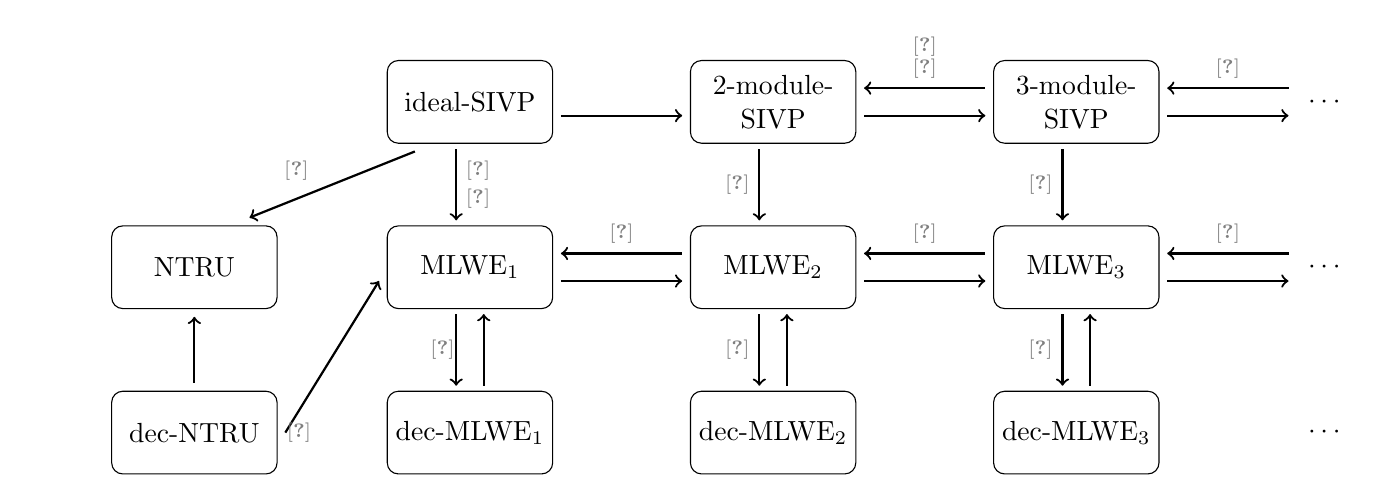
\begin{tikzpicture}[scale = 0.35]

%\begin{scope} %% to crop the picture with a rectangle!
%    \clip(-12,-13) rectangle (30,10);

%% rank 1
\draw[rounded corners] (0, 6) rectangle (6, 9) node[pos=.5,text width=4cm,align=center] {ideal-SIVP};
\draw[rounded corners] (0, 0) rectangle (6, 3) node[pos=.5,text width=4cm,align=center] {MLWE$_1$};
\draw[rounded corners] (0, -6) rectangle (6, -3) node[pos=.5,text width=4cm,align=center] {dec-MLWE$_1$};

\draw[thick,<-] (2.5, 3.2) -- (2.5,5.8);
\draw (2.5,5) node[right, gray] {{\scriptsize \cite{RLWE1}}};
\draw (2.5,4) node[right, gray] {{\scriptsize \cite{RLWE2}}};

\draw[thick,<-] (3.5, -0.2) -- (3.5,-2.8);
\draw[thick,->] (2.5, -0.2) -- (2.5,-2.8);
\draw (2.8,-1.5) node[left, gray] {{\scriptsize \cite{RLWE2}}};

%% rank 2
\draw[rounded corners] (11, 6) rectangle (17, 9) node[pos=.5,text width=4cm,align=center] {$2$-module-\\SIVP};
\draw[rounded corners] (11, 0) rectangle (17, 3) node[pos=.5,text width=4cm,align=center] {MLWE$_2$};
\draw[rounded corners] (11, -6) rectangle (17, -3) node[pos=.5,text width=4cm,align=center] {dec-MLWE$_2$};

\draw[thick,<-] (13.5, 3.2) -- (13.5,5.8);
\draw (13.5,4.5) node[left, gray] {{\scriptsize \cite{MLWE2}}};

\draw[thick,<-] (14.5, -0.2) -- (14.5,-2.8);
\draw[thick,->] (13.5, -0.2) -- (13.5,-2.8);
\draw (13.5,-1.5) node[left, gray] {{\scriptsize \cite{MLWE2}}};


%% rank 3
\draw[rounded corners] (22, 6) rectangle (28, 9) node[pos=.5,text width=4cm,align=center] {$3$-module-\\SIVP};
\draw[rounded corners] (22, 0) rectangle (28, 3) node[pos=.5,text width=4cm,align=center] {MLWE$_3$};
\draw[rounded corners] (22, -6) rectangle (28, -3) node[pos=.5,text width=4cm,align=center] {dec-MLWE$_3$};

\draw[thick,<-] (24.5, 3.2) -- (24.5,5.8);
\draw (24.5,4.5) node[left, gray] {{\scriptsize \cite{MLWE2}}};

\draw[thick,<-] (25.5, -0.2) -- (25.5,-2.8);
\draw[thick,->] (24.5, -0.2) -- (24.5,-2.8);
\draw (24.5,-1.5) node[left, gray] {{\scriptsize \cite{MLWE2}}};

%% etc
\draw (34, 7.5) node {$\cdots$};
\draw (34, 1.5) node {$\cdots$};
\draw (34, -4.5) node {$\cdots$};

%% diagonal arrows
%\draw[thick,->] (6.3, 2.5) -- (10.7,6.5);
%\draw[thick,->] (17.3, 2.5) -- (21.7,6.5);
%\draw[thick,->] (28.3, 2.5) -- (32.7,6.5);

%% horizontal arrows
%% LWE
\draw (8.5,2) node[gray, above] {{\scriptsize \cite{AD17}}};
\draw[thick,<-] (6.3, 2) -- (10.7,2);
\draw[thick,->] (6.3, 1) -- (10.7,1);
\draw (19.5,2) node[gray, above] {{\scriptsize \cite{AD17}}};
\draw[thick,<-] (17.3, 2) -- (21.7,2);
\draw[thick,->] (17.3, 1) -- (21.7,1);
\draw (30.5,2) node[gray, above] {{\scriptsize \cite{AD17}}};
\draw[thick,<-] (28.3, 2) -- (32.7,2);
\draw[thick,->] (28.3, 1) -- (32.7,1);

%% SIVP
\draw[thick,->] (6.3, 7) -- (10.7,7);

\draw[thick,->] (17.3, 7) -- (21.7,7);
\draw[thick,<-] (17.3, 8) -- (21.7,8);
\draw (19.5,8.8) node[above,gray] {{\scriptsize \cite{LPSW19}}};
\draw (19.5,8) node[above,gray] {{\scriptsize \cite{MS20}}};
\draw[thick,->] (28.3, 7) -- (32.7,7);
\draw[thick,<-] (28.3, 8) -- (32.7,8);
\draw (30.5,8) node[above,gray] {{\scriptsize \cite{MS20}}};

%% Big box
%\draw[dotted, rounded corners, thick, gray] (35,10) -- (10,10) -- (10,4) -- (-1,4) -- (-1,-7) -- (36,-7) -- (36,10) -- (35,10);


%% NTRU
\draw[rounded corners] (-10, 0) rectangle (-4, 3) node[pos=.5,text width=4cm,align=center] {NTRU};
\draw[rounded corners] (-10, -6) rectangle (-4, -3) node[pos=.5,text width=4cm,align=center] {dec-NTRU};


%% NTRU arrows
\draw[thick,->] (1, 5.7) -- (-5,3.3);
\draw (-2.5,5) node[left,gray] {{\scriptsize \cite{PS21}}};

\draw[thick,<-] (-7, -0.3) -- (-7,-2.7);

\draw[thick,->] (-3.7, -4.5) -- (-0.3,1);
\draw (-4,-4.5) node[right,gray] {{\scriptsize \cite{Pei16}}};

%\end{scope}

\end{tikzpicture}
}
\end{center}
\caption{PoReductions (possibly quantum) between algebraic variants of lattice problems. Reductions with no references should be immediate.}
\label{fig:reductions}
\end{figure}

Let us comment Figure~\ref{fig:reductions} a bit. A first observation is that the situation seems somewhat different between MLWE and module-SIVP for the rank-$1$ case. Indeed, for MLWE$_1$, we have reductions \emph{from and to} MLWE$_2$, meaning that these two problems are somewhat equivalent. In the case of module-SIVP, we only have the easy reduction from $1$-module-SIVP (i.e., ideal-SIVP) to $2$-module-SIVP. We already discussed in the previous section that the absence of reduction from $2$-module-SVP to ideal-SVP may be due to a gap in the hardness between these two problems.\footnote{The SIVP case is similar to the SVP case here.} For the MLWE problem, we know that the is no such gap between rank-$1$ and rank-$2$. As explained above, this is the reasons why, in these lecture notes, we decided to use the terminology MLWE$_1$ and not RLWE (there is no reason to treat the case $n = 1$ differently from the cases $n \geq 2$).

On a related topic, you may have heard that MLWE$_1$ (i.e., RLWE) is based on the hardness of ideal-SIVP, and that solving ideal-SIVP efficiently would have an impact on the security of MLWE$_1$. This is not really correct. As you can see on the figure, we only have a reduction from ideal-SIVP to MLWE$_1$, so an algorithm solving ideal-SIVP cannot be transformed into an algorithm solving MLWE$_1$ (at least not with our current knowledge). The figure also shows that one can reduce $2$-module-SIVP to the MLWE$_1$ problem (for some range of parameters), so, if you prefer, you could say that the hardness of MLWE$_1$ is based on the hardness of $2$-module-SIVP (which seems safer than ideal-SIVP).

The figure shows that MLWE$_k$ (resp $k$-module-SIVP) is somewhat equivalent to MLWE${k+1}$ (resp $(k+1)$-module-SIVP) for all $k \geq 1$ (resp. $k \geq 2$). These reductions can be combined, but they induce some loss on the parameters each time. Hence, combining many of these reductions would lead to a reduction with a significant loss. For example, there is a polynomial time reduction from $k$-module-SIVP$_\gamma'$ to $2$-module-SIVP$_\gamma$ for large $k$'s, but the parameter $\gamma'$ is of the order of $\gamma^{2k}$: the loss is exponential in $k$.

As a last observation, you may have notices that we know less for the NTRU problem than for the MLWE problem. In particular, an important open question is whether the search and decision versions of the NTRU problem are equivalent or not.\footnote{Some preliminary results have been proven in this direction in~\cite{PS21}: the authors showed equivalence between dec-NTRU and a variant of the search NTRU problem. But the equivalence between this variant of search NTRU and the search NTRU defined in Definition~\ref{def:NTRU} above is still open.}

%explain Martin and Amit's reduction (if it can be done easily)
\paragraph{Albrecht-Deo's reduction.} In these lecture notes, we will not cover the details of all the reductions mentioned in Figure~\ref{fig:reductions}, we refer the reader to the cited articles for more details. We will only detail the reduction by Albrecht and Deo~\cite{AD17}, which shows that MLWE$_{1}$ is no easier than MLWE$_{k}$, for appropriately chosen parameters.

%In order to simplify the statement and the proof, we will consider a variant of the MLWE problem where the error is worst-case, below some bound $B$. In other words, the error $\vec e$ is not sampled anymore from some small distribution $\chi^m$, but is arbitrarily chosen among vectors $\vec e \in R^m$ with $\|\mink(e_i)\| \leq B$ for all their coordinates $e_i$. We write this variant wc-error-MLWE$_{n,m,q,B}$.

%In order to state the result, we need to introduce the Hermite Normal Form variant of the module-LWE problem. In this variant, the secret $\vec s$ is sampled from the same distribution $\chi$ as the error, instead of being chosen uniformly at random in $R_q^n$. More precisely, the Hermite Normal Form search module-LWE problem HNF-MLWE$_{n,m,q,\chi}$ asks, given as input a sample from the module-LWE distribution $A^{\vec s}_{n,m,q,\chi}$ for some $\vec s \leftarrow \chi^n$, to recover the secret vector $\vec s$.
%Recall that one should think of $\chi$ as outputting small elements, so in this version, the secret vector $\vec s$ is also small. This form is usually convenient for proofs, as the one of Albrecht and Deo. Moreover, it was proved by Roux-Langlois and Stehlé~\cite[Le. 4.24]{LS15} that this variant of MLWE is equivalent to the standard MLWE problem, for a well-chosen distribution $\chi$.

In order to simplify the statement, we will introduce $B$-bounded distributions. A distribution $\chi$ over $R$ is said to be $B$-bounded if, for all $x$ in the support of $\chi$, we have $\|\mink(x)\| \leq B$. We are now ready to state a simplified version of Albrecht and Deo's main result from~\cite{AD17}.

\begin{lemma}
\label{lemma:Albrecht-Deo}
Let $\alpha_1, \dots, \alpha_d \in R$ be a known basis of $R$.
Let $q \geq 2$, $m \geq n \geq 2$ and $\chi$ be a $B$-bounded distribution for some $B > 0$. There is a polynomial 
algorithm $\mathcal{A}$ that takes as input $(\vec A, \vec b) \leftarrow A^{\vec s}_{n,m,q,\chi}$ for some $\vec s \leftarrow \chi^n$ and outputs $(\vec{\tilde{a}}, \vec{\tilde{b}}) \in R_{q'}^m \times R_{q'}^m$ where $q' = q^n$ and $\vec{\tilde{b}} = \vec{\tilde{a}} \cdot \tilde{s} + \vec{\tilde{e}} \bmod q'$ for some $\vec{\tilde{e}} \in R^m$ with 
\[\|\mink(\tilde{e}_i) \| \leq B' := 3nd \cdot \max_i \|\mink(\alpha_i)\| \cdot q^{n-1} \cdot B\] 
for all coordinates $\tilde{e}_i$ of $\vec{\tilde{e}}$, and where $\tilde{s} = \sum_{i=1}^n s_i q^{i-1} \in R_{q'}$. Moreover, the vector $\vec{\tilde{a}} \in R_q'^m$ is uniformly distributed.
%time reduction from HNF-MLWE$_{n,m,q,\chi}$ to MLWE$_{1,m,q', \chi'}$, where $q' = q^n$ and $\chi'$ is a $B'$-bounded distribution \emph{depending on the MLWE} for $B' = 2dq^{n-1} \cdot B$.
\end{lemma}
At a high level, the reduction from the lemma transforms a sample from MLWE with secret dimension $n$, modulus $q$ and error bounded by $B$, into a sample from MLWE with secret dimension $1$, modulus $q' = q^n$ and error bounded by $B' = 3nd\cdot \max_i \|\mink(\alpha_i)\| \cdot q^{n-1} \cdot B$. Recall that the interesting parameter regarding the noise size is the noise ratio $\alpha = B/q$. After the reduction, this noise ratio becomes $\alpha' = B'/q' = 3nd \cdot \max_i \|\mink(\alpha_i)\| \cdot  \alpha$. Hence, the noise ratio is increased only slightly by the reduction (by a quantity depending on the number field $K$).\footnote{Note that for cyclotomic fields, we know a basis of $R$ such that $\max_i \|\mink(\alpha_i)\| = \sqrt{d}$.}
Note also that, from the new secret $\tilde{s}$, one can efficiently recover the original secret $\vec s \in R_{q}^n$ be decomposing $\tilde{s}$ in base $q$. So a solution to the new MLWE$_1$ instance can be transformed back into a solution to the original MLWE$_n$ instance.

Let's emphasize that the statement from Lemma~\ref{lemma:Albrecht-Deo} does not immediately provide a reduction from MLWE$_{n,m,q,\chi}$ to MLWE$_{1,m,q',\chi'}$ for some $B'$-bounded distribution $\chi'$. The first obstacle is that the noise term $\tilde{e}$ obtained after the reduction depends on the MLWE instance $(\vec A, \vec b)$ (and in particular on the secret $\vec s$). To transform the tuple $(\tilde{a}, \tilde{b})$ into an MLWE$_{1,m,q',\chi'}$ sample, one would need to make the noise term independent from the input of the reduction. This can be done using a technique called noise sampling, which essentially consists in adding a large fresh noise term to the sample, to hide the old noise term. This works well but requires to take $q$ quite large, since the noise flooding technique will increase $\tilde{e}$ quite a lot.

Another limitation of our lemma is that we assumed that the secret $\vec s$ was sampled from the same distribution $\chi$ as the noise term $\vec e$, whereas in our definition of MLWE the secret $\vec s$ should be uniformly chosen in $(R_q)^n$. The variant of MLWE with small noise is known as the Hermite normal form variant of MLWE, and Roux-Langlois and Stehlé proved that this variant is equivalent to the standard MLWE problem for a well chosen distribution $\chi$~\cite[Le. 4.24]{MLWE2}.

Let us now prove the lemma. \textbf{Do not read the following proof before the tutorial session, since we will do the proof as an exercise.}

\begin{proof}
Let $(\vec A, \vec b)$ be as in the lemma's statement. Then $\vec b = \vec A \cdot \vec s + \vec e \bmod q$ for some $\vec e \leftarrow \chi^m$. Since we assumed that $\chi$ is $B$-bounded, we know that $\|\mink(e_i)\| \leq B$ for all coordinate $e_i$ of $\vec e$. Similarly, since $\vec s \leftarrow \chi^n$, then $\|\mink(s_i)\| \leq B$ for all coordinate $s_i$ of $\vec s$.

For every coordinate $a_{i,j} \in R_q$ of $\vec A$, let us compute a representative $\overline{a}_{i,j} \in R$ such that $\|\mink(a_{i,j}) \| \leq q \cdot d \cdot \max_i \|\alpha_i\|$. To do so, we first compute any representative $x \in R$. Then, we write $x = \sum_i x_i \alpha_i$, with $x_i \in \ZZ$, which is possible since the $alpha_i$'s form a basis of $R$. Finally, we reduce the $x_i$'s module $q$: $\overline{a}_{i,j} = \sum_i y_i \alpha_i$n where $y_i$ is the integer in $[0,q)$ equal to $x_i$ modulo $q$. Note that $\overline{a}_{i,j}$ differs from $x$ by multiples of $q$, so it is another representative of $a_{i,j} \in R_q$. Moreover, $\|\mink(a_{i,j})\| \leq \sum_i |y_i| \cdot \|\mink(\alpha_i)\| \leq q \cdot d \cdot \max_i \|\mink(\alpha_i)\|$ as desired.

Let us now compute $\vec{\tilde{a}} = (\tilde{a_1}, \dots, \tilde{a_m})$ where $\tilde{a_i} = \sum_{j = 1}^n \overline{a}_{i,j} q^{n-j}$. 
We also define $\tilde{b} = q^{n-1} \cdot \vec b \in R^m$.
Recall from the lemma that $\tilde{s}$ is defined as $\tilde{s} = \sum_{j=1}^n s_j q^{j-1}$.

Let us fix some $i \in \{1,\dots,m\}$. We want to prove that $\tilde{b_i} = \tilde{a_i} \cdot \tilde{s} + \tilde{e_i}\bmod q'$ for some small $\tilde{e_i}$. Let us explicit the computation
\begin{align*}
\tilde{a_i} \cdot \tilde{s} &= \Big(\sum_{j = 1}^n \overline{a}_{i,j} q^{n-j} \Big) \cdot \Big( \sum_{j=1}^n s_j q^{j-1}\Big) \\
&= \sum_{k = 0}^{n-1} q^k \cdot \sum_{j = 1}^{k+1} s_j \overline{a}_{i,n-k-1+j} \bmod q^n\\
&= q^{n-1} \cdot \sum_{j = 1}^n s_j \overline{a}_{i,j} + \sum_{k = 0}^{n-2} q^k \cdot \sum_{j = 1}^{k+1} s_j \overline{a}_{i,n-k-1+j} \bmod q^n.
\end{align*}
Observe that $\sum_{j = 1}^n s_j \overline{a}_{i,j} = \langle \vec a_i, \vec s \rangle \bmod q = b_i-e_i \bmod q$, where $\vec a_i$ is the $i$-th line of $\vec A$. Hence, $q^{n-1} \cdot \sum_{j = 1}^n s_j \overline{a}_{i,j} = q^{n-1} \cdot (b_i - e_i) \bmod q^n$.
Let us define 
\[ \tilde{e_i} = q^{n-1} \cdot e_i + \sum_{k = 0}^{n-2} q^k \cdot \sum_{j = 1}^{k+1} s_j \overline{a}_{i,n-k-1+j}.\]
By definition, this noise term satisfies $\tilde{b_i} = \tilde{a_i} \cdot \tilde{s} + \tilde{e_i}\bmod q'$. It remains to bound its size.
\begin{align*}
\|\mink(\tilde{e_i})\| & \leq q^{n-1} \cdot \|\mink(e_i)\| + \sum_{k = 0}^{n-2} q^k \cdot \sum_{j = 1}^{k+1} \|\mink(s_j \overline{a}_{i,n-k-1+j})\| \\
&\leq q^{n-1} \cdot B + \sum_{k = 0}^{n-2} q^k \cdot \sum_{j = 1}^{k+1} \|\mink(s_j)\| \cdot \|\mink(\overline{a}_{i,n-k-1+j})\| \\
&\leq q^{n-1} \cdot B + \sum_{k = 0}^{n-2} q^k \cdot \sum_{j = 1}^{k+1} B \cdot q \cdot d \cdot \max_i \|\mink(\alpha_i)\| \\
&\leq q^{n-1} \cdot B + \sum_{k = 0}^{n-2} q^{k+1} \cdot n \cdot B \cdot d \cdot \max_i \|\mink(\alpha_i)\| \\
&\leq q^{n-1} \cdot B + nd \cdot B \cdot \max_i \|\mink(\alpha_i)\| \cdot \frac{q^{n}-1}{q-1} \\
&\leq q^{n-1} \cdot B + nd \cdot B \cdot \max_i \|\mink(\alpha_i)\| \cdot 2q^{n-1},
\end{align*}
where in the last inequality we used the fact that $q \geq 2$ so that $(q-1)^{-1} \leq 2/q$. This provides the desired upper bound on the size of the coordinates of $\vec{\tilde{e}}$.
\end{proof}




\subsection{Cryptographic constructions}
\label{sec:constructions}

\subsection{Cryptanalysis}
\label{sec:cryptanalysis}

%\subsection{Ring and Module variants of LWE, and the NTRU problem}

%Alice -- Réseaux algébriques en cryptographie -- CM: 3h / TD: 1h30

%Ce cours sera consacré au variantes algébriques des problèmes LWE et SIS (définis dans le cours de Adeline Roux-Langlois). En plus des variantes algébriques de LWE et SIS, nous parlerons aussi du problème NTRU, qui n'a pas d'équivalent non-algébrique.
%Le cours sera divisé en trois parties:
%- nous commencerons par définir les variantes algébriques de LWE/SIS et le problème NTRU, et nous parlerons du lien entre ces problèmes et les réseaux (algébriques);
%- nous verrons ensuite comment construire des primitives cryptographiques simples à partir de ces problèmes algorithmiques;
%- enfin, nous parlerons de cryptanalyse et nous présenterons quelques attaques qui exploitent la structure algébrique de ces problèmes.